\documentclass[withoutpreface,bwprint]{cumcmthesis} %去掉封面与编号页
\title{《数据库系统》课程设计报告}
\author{18340206张德龙 \\
	zhangdlong3@mail2.sysu.edu.cn \\
		18340207张昊熹 \\ 
		zhanghx66@mail2.sysu.edu.cn
}
\date{\today}
\usepackage[cache=false]{minted}
\usepackage{diagbox}
%\usepackage{fancyhdr}
%\pagestyle{empty} 
{\renewcommand\fcolorbox[4][]{\textcolor{cyan}{\strut#4}} %屏蔽汇编语言mint的错误
\graphicspath{{figure/}}

\let\algorithm\relax  
\let\endalgorithm\relax 
\usepackage[linesnumbered,ruled,lined]{algorithm2e}
\usepackage{algpseudocode}  
\renewcommand{\algorithmicrequire}{\textbf{Inc\_puct:}}   
\renewcommand{\algorithmicensure}{\textbf{Output:}}   
\SetKwFor{For}{for}{do}{endfor}
\newcommand{\ret}{\textbf{return}}   
\usepackage{ulem}

\makeatletter
\newenvironment{breakablealgorithm}
{% \begin{breakablealgorithm}
	\begin{center}
		\refstepcounter{algorithm}% New algorithm
		\hrule height.8pt depth0pt \kern2pt% \@fs@pre for \@fs@ruled
		\renewcommand{\caption}[2][\relax]{% Make a new \caption
			{\raggedright\textbf{\ALG@name~\thealgorithm} ##2\par}%
			\ifx\relax##1\relax % #1 is \relax
			\addcontentsline{loa}{algorithm}{\protect\numberline{\thealgorithm}##2}%
			\else % #1 is not \relax
			\addcontentsline{loa}{algorithm}{\protect\numberline{\thealgorithm}##1}%
			\fi
			\kern2pt\hrule\kern2pt
		}
	}{% \end{breakablealgorithm}
		\kern2pt\hrule\relax% \@fs@post for \@fs@ruled
	\end{center}
}
\makeatother

\newcounter{Emp}[subsubsection]	% 设置计数器
\newcommand{\kuohao}[1]{ \noindent (#1)}

\usepackage{amssymb}% http://ctan.org/pkg/amssymb
\usepackage{pifont}% http://ctan.org/pkg/pifont
\newcommand{\cmark}{\ding{51}}%
\newcommand{\xmark}{\ding{55}}%
\newcommand{\yuan}{\ding{109}}%

\usepackage{threeparttable}
\setcounter{tocdepth}{3}

\begin{document}
	\maketitle 
%{
%	\centering \kaishu 数据科学与计算机学院 \\
%	 计科 18340206张德龙 \quad \quad \quad \quad 计科 18340207张昊熹 \\
%	 zhangdlong3@mail2.sysu.edu.cn  \quad zhanghx66@mail2.sysu.edu.cn\\
%} 
\begin{table}[H]
\centering
\label{tab:my-table}
\begin{threeparttable}
\begin{tabular}{|c|c|c|c|}
\hline
\textbf{题目} & \multicolumn{3}{c|}{人事工资管理系统的设计}        \\ \hline
\textbf{姓名} & \textbf{学号} & \textbf{班级} & \textbf{分工} \\ \hline
张德龙         & 18340206    & 教务3班        & xxx         \\ \hline
张昊熹         & 18340207    & 教务3班        & xxx         \\ \hline
\end{tabular}
\begin{tablenotes}
%    \footnotesize
    \centering
    \item 提交时间: 2021  年  1    月   10    日
   % \item[**] my website is ... %此处加入注释**信息
\end{tablenotes}
\end{threeparttable}
\end{table}

%\begin{abstract}
%	在本次实验中,我们实现了结合神经网络的蒙特卡洛树搜索算法——即Alpha Zero强化学习算法。并且,在实现了基础的Alpha Zero算法之上,我们通过将代码cython化、使用数据增强、将棋盘正则化等方式对模型进行了改进,在训练了120个epoch后,我们实现的模型对阵随机玩家基本能够达到百分百的胜率,对阵仿真次数比自己多一倍的纯蒙特卡洛搜索玩家也能够达到百分之七十六的胜率,证实了我们实现模型的有效性。
%	
%	\keywords{强化学习 \quad 蒙特卡洛树搜索 \quad  AlphaZero \quad cython \quad 数据增强 }
%\end{abstract}
%
%\tableofcontents

\section{开发环境与开发工具}
1、操作系统:Windows 10;

2、DBMS :mysql 8.0.21;

3、编程环境:Java Development Kit 13.0.1;

4、数据库JDBC接口:mysql-connector-java-8.0.22;

5、开发IDE:IDEA 2020.2.4。
\section{系统需求分析}

企业可以通过人事工资管理系统实现对企业人员信息及工资信息的管理,该系统具有一定的人事档案管理功能。经过调研,对企业进行人事工资事务的管理流程、题设要求进行分析,本实验设计的人事工资管理系统具有如下功能:
\begin{enumerate}
	\item 系统的用户管理:包括普通员工、财务管理员、领导管理员的添加、删除,密码修改等;
	\item 员工的信息管理:包括员工基本信息的查询、添加、删除、修改等;
	\item 员工的考勤管理:包括员工考勤情况的查询、添加、删除、修改等;
	\item 部门的信息管理:包括部门的查询、添加、删除、修改等;
	\item 员工的薪资管理:包括薪资的计算、查询、修改等;
	\item 薪资的统计报表:包括企业薪资、部门薪资、职工薪资的查询等;
\end{enumerate}

数据字典是系统中各类数据描述的集合,是
进行详细的数据收集和数据分析所获得的主要成果。教材中定义的数据字典通常包括数据项、数据结构、数据流、数据存储和处理过程5个部分。本次实验中我们小组设计的数据字典如下:

\subsection{主要数据项}
\begin{table}[H]
\centering
\caption{数据项表}
\begin{tabular}{cccc}
\hline
\textbf{名称} & \textbf{别名} & \textbf{描述}       & \textbf{定义} \\ \hline
姓名          & 名字          & 员工/部门等实体的名字       & 16字符变长字符串   \\ \hline
性别          & -           & 员工的性别             & 2字符变长字符串    \\ \hline
编号          & id、编码       & 系统内各对象的唯一标识符      & 8字符变长字符串    \\ \hline
底薪          & 最低工资        & 一个部门下员工一个月获得的最低工资 & 整型          \\ \hline
职务薪资        & 职薪          & 在部门下所任职务的薪资       & 整型          \\ \hline
税费          & 税费记录        & 员工需要交纳的税务费用       & 整型          \\ \hline
部门人数        & -           & 一个部门所有员工的数目       & 整型          \\ \hline
时间          & -           & 记录时间              & datetime类型  \\ \hline
考勤状态        & 考勤          & 记录考勤的状态           & 8字符变长字符串    \\ \hline
密码          & password    & 登录管理系统需要的密码       & 32字符变长字符串   \\ \hline
权限          & 权限级别        & 在管理系统中具有的权限       & 32字符变长字符串   \\ \hline
            &             &                   &             \\ \hline
\end{tabular}
\end{table}

\subsection{主要数据结构}
\begin{table}[H]
\centering
\caption{数据结构表}
\label{t2}
\begin{tabular}{ccc}
\hline
\textbf{名称} & \textbf{描述}  & \textbf{定义}         \\ \hline
考勤信息        & 考勤信息的整合      & 考勤状态+时间+编号+员工编号     \\ \hline
员工信息        & 存储员工的信息      & 姓名+性别+编号            \\ \hline
部门信息        & 存储部门相关信息     & 人数+底薪+名称+编号         \\ \hline
管理员信息       & 存储管理系统的管理员信息 & 姓名+密码+权限+编号         \\ \hline
职务信息        & 存储员工职务相关信息   & 职务薪资+职务名称+员工编号+部门编号 \\ \hline
            &              &                     \\ \hline
\end{tabular}
\end{table}
\subsection{主要数据流}
\kuohao{1} 员工信息变更数据流:
\begin{itemize}
\item 说明:员工信息的变更产生的数据流向;
\item 数据流来源:员工信息变动事务;
\item 数据流去向:人事管理事务、薪资结算事务;
\item 平均流量:每月一次;
\item 高峰期流量:每月十几次。
\end{itemize}

\kuohao{2} 考勤信息变更数据流:
\begin{itemize}
\item 说明:考勤信息的变更产生的数据流向;
\item 数据流来源:日常考勤事务;
\item 数据流去向:人事管理事务、薪资结算事务;
\item 平均流量:每天几百次;
\item 高峰期流量:每天几千次。
\end{itemize}


\kuohao{3} 部门信息变更数据流:
\begin{itemize}
\item 说明:考勤信息的变更产生的数据流向;
\item 数据流来源:部门信息变更事务;
\item 数据流去向:人事管理事务、薪资结算事务;
\item 平均流量:每月一次;
\item 高峰期流量:每月十几次。
\end{itemize}

\subsection{数据存储}
\kuohao{1} 考勤信息表:
\begin{itemize}
\item 说明:考勤信息的整合;
\item 数据结构:考勤信息;
\item 数据量:一天约100 $\times$ 32 = 3200字节。
\end{itemize}

\kuohao{2} 员工信息表:
\begin{itemize}
\item 说明:员工信息的整合;
\item 数据结构:员工信息;
\item 数据量:约100 $\times$ 32 = 320字节 。
\end{itemize}

\kuohao{3} 部门信息表:
\begin{itemize}
\item 说明:部门信息的整合;
\item 数据结构:部门信息;
\item 数据量:约10 $\times$ 32 = 320字节 。
\end{itemize}

\kuohao{4} 管理员信息表:
\begin{itemize}
\item 说明:管理员信息的整合;
\item 数据结构:管理员信息;
\item 数据量:约10 $\times$ 32 = 320字节 。
\end{itemize}

\kuohao{5} 职务信息表:
\begin{itemize}
\item 说明:职务信息的整合;
\item 数据结构:职务信息;
\item 数据量:约100 $\times$ 64 = 6400字节 。
\end{itemize}

\subsection{主要处理过程}

处理过程名:实时计算薪资。

\begin{itemize}
\item 说明:因为税费、员工信息的不断变更,需要能根据信息实时计算薪资;
\item 输入:员工信息表、部门信息表、职务信息表、时间;
\item 输出:员工薪资表;
\item 处理:结合员工的考勤、职务。部门、税费、输入的时间自动求出工资。
\end{itemize}



\section{功能需求分析}

企业人事工资管理系统按照上面所述,管理功能的需求比较清晰,主要实现了对员工、部门、员工的考勤、员工的薪资等的管理。系统功能模块如图\ref{gongneng}所示。 \par 
	其中“信息管理”板块中的每一个功能管理想都包括查看、添加、删除和修改能功能。
\begin{figure}[H]
    \centering
    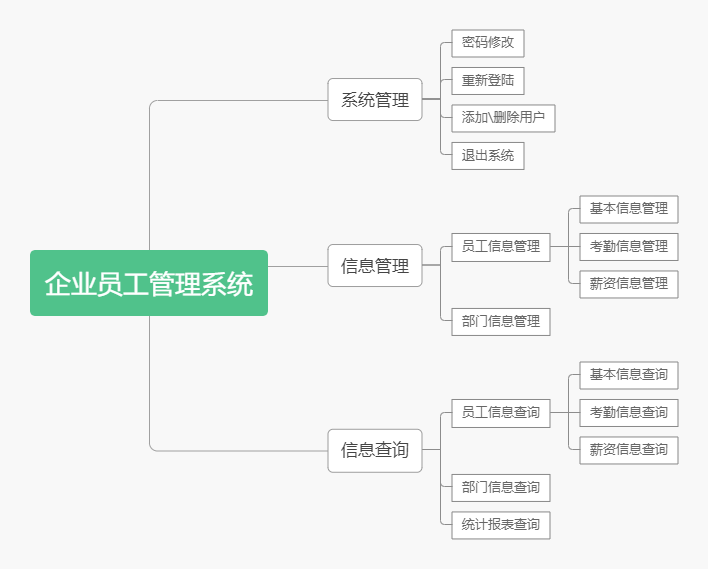
\includegraphics[width=1\linewidth]{gongneng1}
    \caption{系统功能模块图}
    \label{gongneng}
\end{figure}
\section{系统设计}
\subsection{数据概念结构设计}
\begin{enumerate}
	\item 数据流程图。如图\ref{shuju}所示。
	\item 系统ER图。经调研分析后,得人事工资管理系统整体基本ER图如图xxx所示;
	\item Mysql中的加强ER图(EER图),通过ER图使用mysql建立的加强版本的ER图如下所示。
\end{enumerate}
\begin{figure}[H]
    \centering
    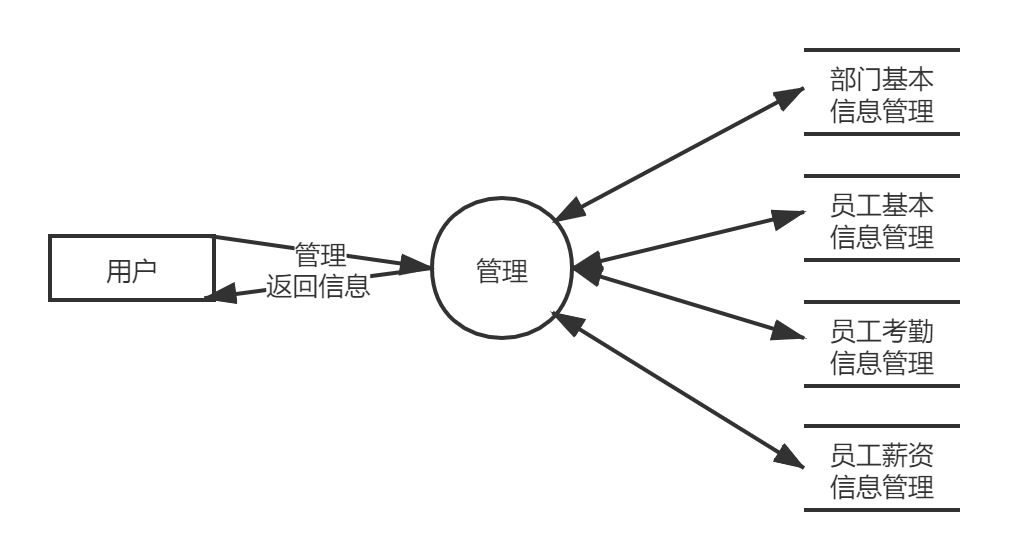
\includegraphics[width=1\linewidth]{shuju}
    \caption{系统功能模块图}
    \label{shuju}
\end{figure}

xx


xx


\subsection{数据库关系模式设计}
按照ER图到逻辑关系模式的转换规则,可得到系统如下x个关系。
\begin{enumerate}
	\item 员工信息(\uline{员工编号},姓名,性别);
	\item 部门信息(\uline{部门编号},名称,底薪,人数);
	\item 管理信息(\uline{职务薪资},职务名称,\uline{部门编号},\uline{员工编号});
	\item 考勤信息(\uline{时间},考勤状态,\uline{员工编号});
	\item 
\end{enumerate}


\subsection{数据库物理结构设计}
本系统数据库表的物理设计通过使用mysql workbench的EER图导出的创建表SQL命令来实现,根据ER图建立的EER关系模型如下:

生成的创建数据库表的SQL命令主要部分如下:
\begin{lstlisting}[language=SQL]
CREATE TABLE IF NOT EXISTS `EnterpriseDB`.`Management` (
  `salary` INT NULL,
  `job` VARCHAR(16) NOT NULL,
  `department_id` VARCHAR(8) NOT NULL,
  `worker_id` VARCHAR(8) NOT NULL,
  PRIMARY KEY (`job`, `department_id`, `worker_id`))
ENGINE = InnoDB;
\end{lstlisting}


\subsection{主要创新点}

为了加强性能、更好地完成客户需求,在系统的设计中我们使用学习到的数据库知识在实验基础的要求上进行了创新:

%\subsubsection{防sql注入攻击}

\subsubsection{设置了多个触发器}
为了实现数据库的完整性约束、自动更新等需求,在本次实验中我们对相关表设置了多个触发器实现了如下需求:

\kuohao{1} 对变量进行完整性约束:

例如,考勤状态必须为正常/迟到/缺勤/请假之一,需要设置如下触发器保证完整性:
\begin{lstlisting}[language=SQL]
CREATE DEFINER = CURRENT_USER TRIGGER `EnterpriseDB`.`Attendence_BEFORE_INSERT` BEFORE INSERT ON `Attendence` FOR EACH ROW
BEGIN
	if new.state != '正常' and new.state != '迟到' 
    and new.state != '缺勤' and new.state != '请假'
	then signal sqlstate '45000'
    set message_text = '状态必须为正常/迟到/缺勤/请假之一';
	end if;
END
CREATE DEFINER = CURRENT_USER TRIGGER `EnterpriseDB`.`Attendence_BEFORE_UPDATE` BEFORE UPDATE ON `Attendence` FOR EACH ROW
BEGIN
	if new.state != '正常' and new.state != '迟到' 
    and new.state != '缺勤' and new.state != '请假'
	then signal sqlstate '45000'
    set message_text = '状态必须为正常/迟到/缺勤/请假之一';
	end if;
END
\end{lstlisting}
其余的完整性约束如性别必须为男或女也在为相应表设置了触发器。

\vspace{1em}
\kuohao{2} 对于数据的自动更新:

在插入/删除某个员工信息后,我们希望能够在相应部门的部门人数数据项进行更改,因此我们设置了如下触发器进行实现:
\begin{lstlisting}[language=SQL]
CREATE DEFINER = CURRENT_USER TRIGGER `EnterpriseDB`.`Management_BEFORE_INSERT` BEFORE INSERT ON `Management` FOR EACH ROW
BEGIN
	if new.department_id not in (select id from Department)
	then signal sqlstate '45000'
    set message_text = '员工部门信息输入错误——不存在的部门';
	end if;
    update Department set member_num = member_num + 1 where id = new.department_id;
END
CREATE DEFINER = CURRENT_USER TRIGGER `EnterpriseDB`.`Management_BEFORE_DELETE` BEFORE DELETE ON `Management` FOR EACH ROW
BEGIN
	update Department set member_num = member_num - 1 where id = old.department_id;
END
\end{lstlisting}
注意到员工调整部门(更新操作)需要对两个部门的人数进行更改:
\begin{lstlisting}[language=SQL]
CREATE DEFINER = CURRENT_USER TRIGGER `EnterpriseDB`.`Management_BEFORE_UPDATE` BEFORE UPDATE ON `Management` FOR EACH ROW
BEGIN
	if new.department_id not in (select id from Department)
	then signal sqlstate '45000'
    set message_text = '员工部门信息输入错误——不存在的部门';
	end if;
    update Department set member_num = member_num + 1 where id = new.department_id;
	update Department set member_num = member_num - 1 where id = old.department_id;
END
\end{lstlisting}

\subsubsection{建立视图}
优点:封装细节

如果雾化提升性能
\subsubsection{建立存储过程}

通过建立存储过程便于调用

\subsubsection{创建索引}

根据数据字典中对于 xx的分析可得,对于的xxx的查询会较为频繁 
因此为xxx是使用如下语句创建索引
\begin{lstlisting}[language=SQL]
xxx
\end{lstlisting}
从而使得对于xxx的查询更为高效。

\section{系统功能的实现}

\subsection{数据库连接通用模块}

要使得应用程序能够与数据库通信,首先需要构建数据库连接的通用模块。

\subsubsection{实现思想}
JDBC标准定义了Java程序连接数据库服务器的应用程序接口,通过查询Mysql官网提供的手册\url{https://dev.mysql.com/doc/connector-j/8.0}来实现数据库的连接。

\vspace{1em}

\kuohao{1} 连接到数据库:

首先建立一个通过调用DriverManager类的getConnection方法来打开一个数据库连接:
\begin{lstlisting}[language=java]
Class.forName("com.mysql.cj.jdbc.Driver");
conn = DriverManager.getConnection("jdbc:mysql://localhost:3306" + "/" + ConfigIni.DBName +
        "?" + "user=" + ConfigIni.user + "&password=" + ConfigIni.passwd + "&serverTimezone=UTC");
\end{lstlisting}

\kuohao{2} 向数据库中传递SQL语句:

对执行查询、更新等SQL语句的方法进行了封装,便于获取需要的结果。更新类SQL语句需要获取执行是否成功的结果,JDBC设置为int类型;查询类SQL语句执行返回值为ResulSet结果集类型,并且在执行更新语句完毕后可以将statement释放。执行更新类SQL语句的关键代码如下,对查询类SQL命令的封装类似:
\begin{lstlisting}[language=java]
// 执行更新类SQL命令的函数
public static int executeUpdate (String sql) {
    int i= 0;
    try {
        stmt = conn.createStatement (ResultSet. TYPE_SCROLL_SENSITIVE,
        ResultSet. CONCUR_READ_ONLY);
        i = stmt.executeUpdate (sql);
        //conn.commit ();
    }
    catch(Exception e) {
        e.printStackTrace();
    }
    finally {
        free_Stmt(stmt);
    }
    return i;
}
\end{lstlisting}

\vspace{1em}
\kuohao{3} \textbf{防SQL注入}——使用预备语句:

在查询手册的时候调查到,使用预备语句能够有效地防止SQL注入攻击。因此,在数据库连接中我们封装了使用预备语句的接口便于调用,其中封装的执行查询预备语句的函数如下:
\begin{lstlisting}[language=java]
// 执行查询预备SQL命令,返回记录集对象函数
    public static ResultSet executeQuery (PreparedStatement stmt) throws SQLException{
        try {
            rs= stmt.executeQuery();
        }catch(SQLException ex) {
            handleSQLException(ex);
            throw ex;
        }
        // 注意:free statement 会也会close result
        return rs;
    }
\end{lstlisting}

\noindent
预备语句的使用举例如下:
\begin{lstlisting}[language=java]
String sql = "SELECT * FROM Administrator WHERE name=? AND passwd=?";
// 防注入攻击
// 预编译
PreparedStatement stmt = Connector.conn.prepareStatement(sql);
//设置参数
stmt.setString(1, user);
stmt.setString(2, passwd);
// 执行
ResultSet rs = Connector.executeQuery(stmt);
\end{lstlisting}
其中setString方法会将用户输入的符号进行转义,有效地防止了SQL注入攻击。

\vspace{1em}
\kuohao{4} 其余辅助函数:

我们编写的数据库连接类还封装了许多辅助函数便于后续功能的调用,其中关键辅助函数的签名如下:
\begin{lstlisting}[language=java]
// 打印SQL语句执行中的问题
private static void handleSQLException(SQLException ex)
// 关闭Connector
public static void close()
// 释放结果集
private static void free_Res(ResultSet rs)
// 释放语句
public static void free_Stmt(Statement stmt)
// 获取结果集的行数
public static int getRowCnt(ResultSet rs)
\end{lstlisting}

\subsection{登陆界面模块}

\subsubsection{实现思想}
核心思想使用上述封装的Connector连接数据库,然后通过调用预备语句
\begin{lstlisting}[language=SQL]
SELECT * FROM Administrator WHERE name=? AND passwd=?
\end{lstlisting}
来查询是否输入了在数据库中存储的用户名和密码,关键代码如下:
\begin{lstlisting}[language=java]
String sql = "SELECT * FROM Administrator WHERE name=? AND passwd=?";
// 防注入攻击
// 预编译
PreparedStatement stmt = Connector.conn.prepareStatement(sql);
// 设置参数
stmt.setString(1, user);
stmt.setString(2, passwd);
// 执行
ResultSet rs = Connector.executeQuery(stmt);
if(rs.next())
{
    System.out.println("密码正确");
    jf.setVisible(false);
    Main mainPage = new Main(); //开始主题运行界面
    mainPage.main(new String [] {});
}		
\end{lstlisting}


\subsubsection{运行界面}
密码输入界面如下:
\begin{figure}[H]
	\centering
	\begin{minipage}[t]{0.3\linewidth}
		\centering
		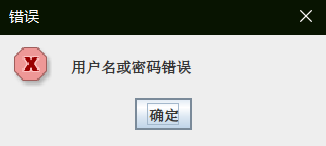
\includegraphics[width=1\linewidth]{login2}
		\caption{密码错误提示}
	\end{minipage}
	\begin{minipage}[t]{0.29\linewidth}
		\centering
		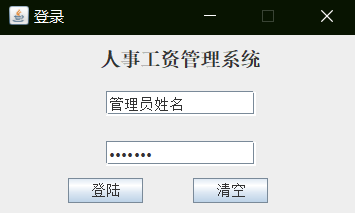
\includegraphics[width=1\linewidth]{login1}
		\caption{密码输入界面}
	\end{minipage}
	\begin{minipage}[t]{0.3\linewidth}
		\centering
		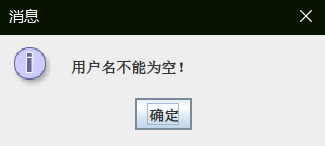
\includegraphics[width=1\linewidth]{login3}
		\caption{密码不能为空}
	\end{minipage}
\end{figure}
密码输入正确后,进入主界面模块。

\subsection{主界面模块}

\subsubsection{实现思想}


\subsubsection{运行界面}

\section{实验总结}

在本次实验中,我们实现了。

在训练过程中,

除了使用cython对数据采样本身进行加速外,

在对弈过程中,


在本次实验中,

通过本次实验,我们对于马尔可夫决策过程、贝尔曼方程等相关知识的理解更为深刻;对于蒙特卡洛树搜索、代码的cython实现、棋盘的正则化等相关过程更为熟悉;对于前沿的强化学习知识——基于蒙特卡洛树搜索与神经网络的Alpha Zero算法有了更深的体会……总而言之,收获颇丰。



%\begin{table}[H]
%\centering
%\caption{实验结果}
%\begin{threeparttable}
%\begin{tabular}{cccc}
%\hline
%      & Y-搜索总结点数 & N-搜索总结点数 &  搜索结点下降百分比 \\ \hline
%随机排序   &   88556      &  122451   & 27.68 \\ 
%行棋排序 &    5842     &  14312  & \textbf{59.18} \\ 
%行棋排序+向前剪枝 &   \textbf{1631}     &     3617   &  54.91 \\ \hline
%\end{tabular}
%\begin{tablenotes}
%    \footnotesize
%    \centering
%    \item[注:]  Y-表示使用置换表,N-表示不使用置换表。
%   % \item[**] my website is ... %此处加入注释**信息
%\end{tablenotes}
%\end{threeparttable}
%\end{table}

%\begin{figure}[H]
%	\centering
%	\begin{minipage}[t]{0.29\linewidth}
%		\centering
%		\includegraphics[width=1\linewidth]{zeve1}
%		\caption{随机排序}
%	\end{minipage}
%	\begin{minipage}[t]{0.3\linewidth}
%		\centering
%		\includegraphics[width=1\linewidth]{zeve2}
%		\caption{行棋排序}
%	\end{minipage}
%	\begin{minipage}[t]{0.3\linewidth}
%		\centering
%		\includegraphics[width=1\linewidth]{zeve3}
%		\caption{行棋排序+剪枝}
%	\end{minipage}
%\end{figure}

%\maketitle
%\begin{abstract}
%	摘要
%	\keyword key
%\end{abstract}

%\inputminted{makefile}{./code/exec.sh}

%\begin{minted}{gas}
%	code
%\end{minted}

%\begin{figure}[H]
%	\centering
%	\includegraphics[width=0.8\linewidth]{1}
%	\caption{caption}
%\end{figure}

%\begin{thebibliography}{99}
%	\bibitem{1}  基于模拟的搜索与蒙特卡罗树搜索(MCTS)——\url{https://www.cnblogs.com/pinard/p/10470571.html}
%	\bibitem{3} AlphaGo Zero强化学习原理——\url{https://www.cnblogs.com/pinard/p/10609228.html}
%	\bibitem{4} 马尔科夫决策过程(MDP)——\url{https://www.cnblogs.com/pinard/p/9426283.html}
%	\bibitem{2} Alpha Zero初探——\url{https://www.hhyz.me/2018/08/08/AlphaGO-Zero}
%	\bibitem{Alpha Z} Silver D , Schrittwieser J , Simonyan K , et al. Mastering the game of Go without human knowledge[J]. Nature, 2017, 550(7676):354-359.
%%	\bibitem{3} Alpha Zero 教程——\url{https://github.com/junxiaosong/AlphaZero_Gomoku}
%%	\bibitem{4} Alpha Zero 教程——\url{https://github.com/bhansconnect/alpha_zero_othello}
%%	\bibitem{5} Apl
%\end{thebibliography}
%
%\begin{appendices}
%	\section{组员分工}
%	\begin{table}[H]
%		\centering
%		\caption{分工明细}
%		\label{tab:F1}
%		\begin{tabular}{l|l|l|l}
%			\hline
%			& \multicolumn{3}{c}{\textbf{分工}}                                                                                                                   \\ \hline
%			\textbf{张德龙} & \multicolumn{3}{l}{\begin{tabular}[c]{@{}l@{}}负责模型原理设计、模型代码的主要实现、辅助函数实现、报告编写。
%		
%			\end{tabular}} \\ \hline
%			\textbf{张昊熹} & \multicolumn{3}{l}{\begin{tabular}[c]{@{}l@{}}负责模型原理设计、模型代码实现、辅助函数主要实现、报告编写。
%			\end{tabular}}                                  \\ \hline
%
%		\end{tabular}
%	\end{table}
%\end{appendices}

\end{document}